\documentclass [a4paper ] {report}
\usepackage{graphicx}
\usepackage{amsmath}
\DeclareMathOperator{\taninv}{tan\,inverse}


\begin{document}


\title{Project Report\\On\\Four Legged Walking Robot }
\author{Sakib Saleh\\ID:160203020009\\ 
Supervised\\By\\Noushad Sojib\\
Head,Dept. of CSE\\North East University Bangladesh\\
Course Code: CSE 400}
\date{\today}
\maketitle
\tableofcontents
\newpage
\listoffigures
\newpage
\begin{center}

\abstractname{\\

In this project I will build a simple four legged robot which will be able to walk.And every legs of this robot will have two degrees of freedom(2DOF).First of all I will simulate the dummy robot on v-rep simulator.If i can complete the simulation on v-rep and if it's able to walk on plain surface.Then I will work on hardware part.In hardware part I will implement the same method that I have already applied on the dummy robot on v-rep simulator. 


}



\end{center}

\newpage
\section{Introduction}
Four legged robot is a type of mobile robot which use articulated limbs, such as leg mechanism to provide motion.
Legged robots often imitate animals such as human or animal.There is a example of a four legged robot is given bellow.

\begin{center}
Mini cheetah Which is developed by MIT\vadjust{\vskip 10mm \vskip 0pt}
\begin{figure}[h]
\begin{center}
  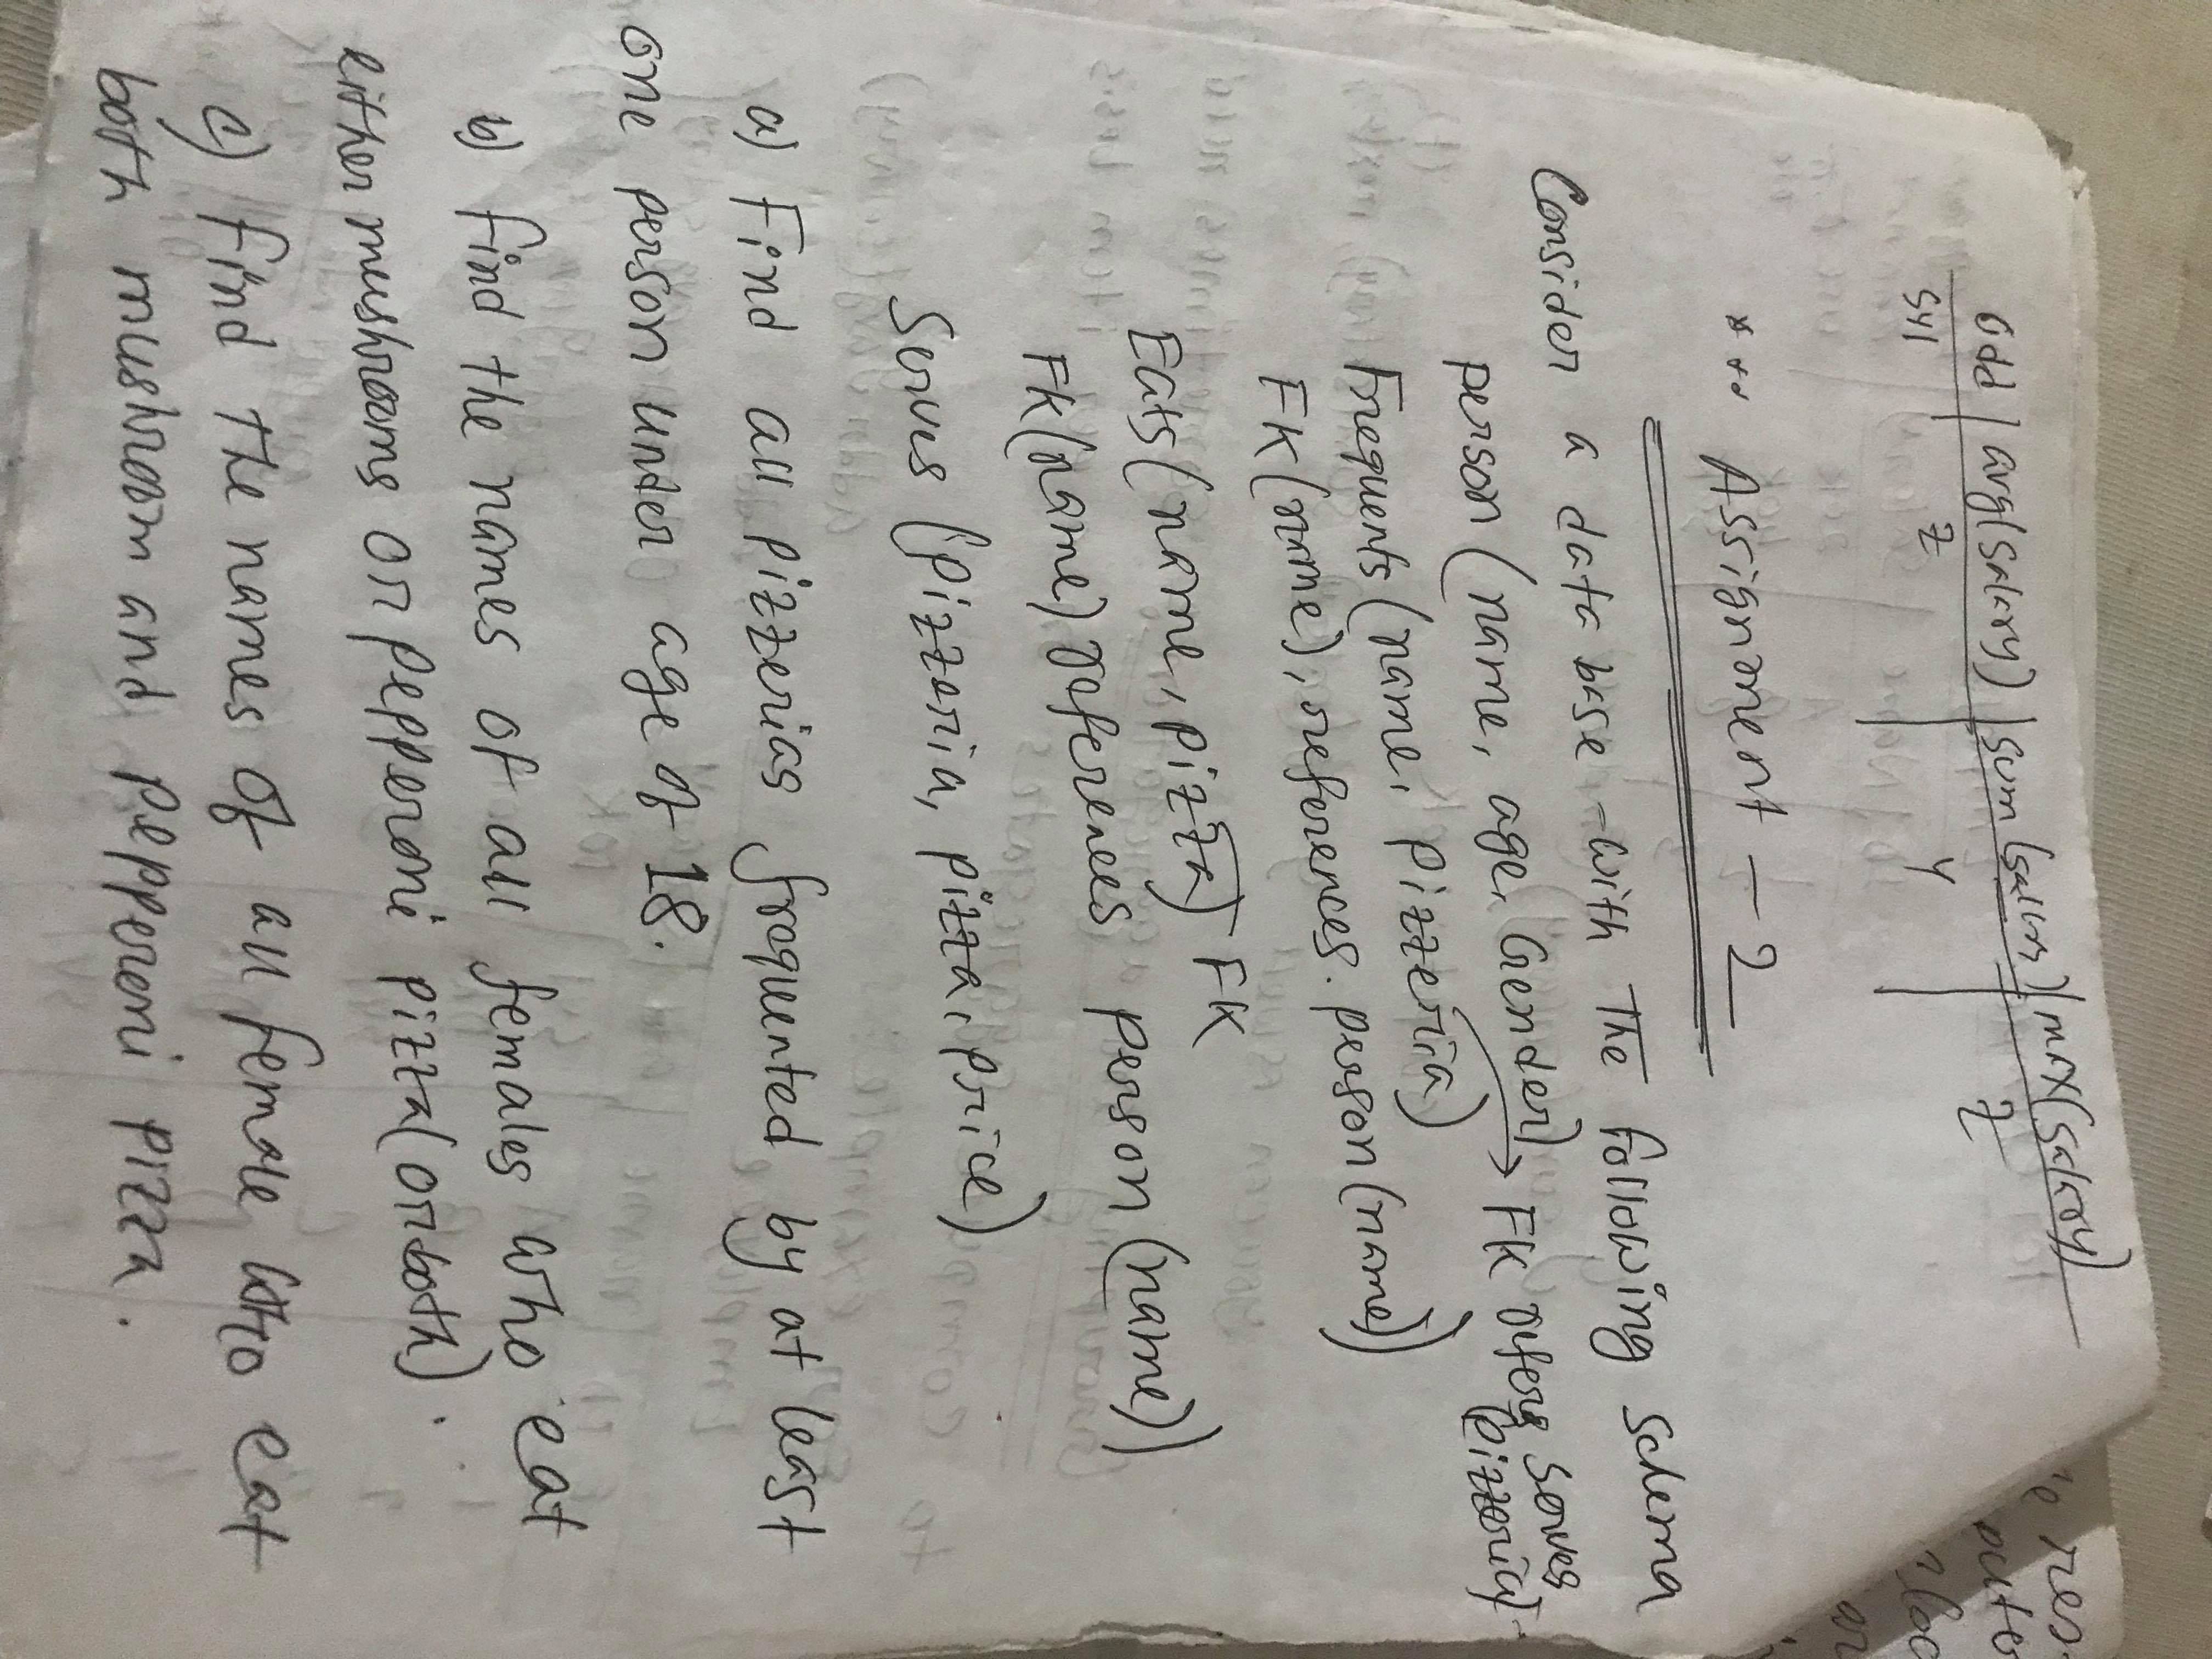
\includegraphics[scale=.3]{1.jpg}
\end{center}
  \caption{Image of Mini Cheetah \vadjust{\vskip 10mm \vskip 0pt}}
\label{fig:fig2}
\end{figure}
\end{center}
\hfill \break
\subsection{Purpose}
Legged robot can be used in rescue mission.Legged robots are mobile robots that use mechanical limbs for movement, they are similar to wheeled robots, but their locomotion methods are more complicated compared to their wheeled counterparts, they perform much better than wheeled robots on uneven terrain.So it can easily complete a task which is tough for wheeled robot or human. 
\subsection{Known four legged robots}
\begin{itemize}
\item MIT Cheetah
\item MIT Mini Cheetah 
\item Spot Boston Dynamics
\item Doggo 
\end{itemize}
These are the famous four legged robot, and those are developed by Massachusetts Institute of Technology,Boston University and Stanford University

\newpage

\section{Kinematics}

Kinematics is a branch of classical mechanics that describes the motion of points, bodies (objects), and systems of bodies (groups of objects) without considering the forces that cause them to move. Kinematics, as a field of study, is often referred to as the "geometry of motion" and is occasionally seen as a branch of mathematics.
\subsection{Forward Kinematics}
Forward kinematics refers to the use of the kinematic equations of a robot to compute the position of the end-effector from specified values for the joint parameters. The kinematics equations of the robot are used in robotics, computer games, and animation.\\
Forward Kinematics Equation for 2DOF(two Degree of freedom) leg\\
\begin{equation}
x=l1\cos\theta1+l2\cos(\theta1+\theta2)
\end{equation}

\begin{equation}
x=l1\sin\theta1+l2\sin(\theta1+\theta2)
\end{equation}

\subsection{Inverse Kinematics}
Inverse kinematics is an example of the kinematic analysis of a constrained system of rigid bodies, or kinematic chain. The kinematic equations of a robot can be used to define the loop equations of a complex articulated system. These loop equations are non-linear constraints on the configuration parameters of the system.
Inverse Kinematics Equation for 2DOF(two Degree of freedom) leg\\

\begin{equation}
r=(x*x)+(y*y)
\end{equation}

\begin{equation}
\alpha=\taninv\frac{y}{x}
\end{equation}

\begin{equation}
\beta=\cos inverse(((r*r)+(l1*l1)-(l2*l2))/(2*r*l1))
\end{equation}

\begin{equation}
Joint1=\alpha-\beta
\end{equation}
\begin{equation}
joint2=\cos inverse(((x*x)+(y*y)-(l1*l1)-(l2*l2))/(2*l1*l2))
\end{equation}
\newpage


\subsection{Use of Forward Kinematics on my project}
First of all I have create a 2dof leg on v-rep simulator, then i write a java code to implement the forward kinematics on this leg by using graphical user interface.By using forward kinematics i can move this leg to x axis and y axis.








\begin{center}
 leg design on v-rep simulator\vadjust{\vskip 10mm \vskip 0pt}
\begin{figure}[h]
\begin{center}
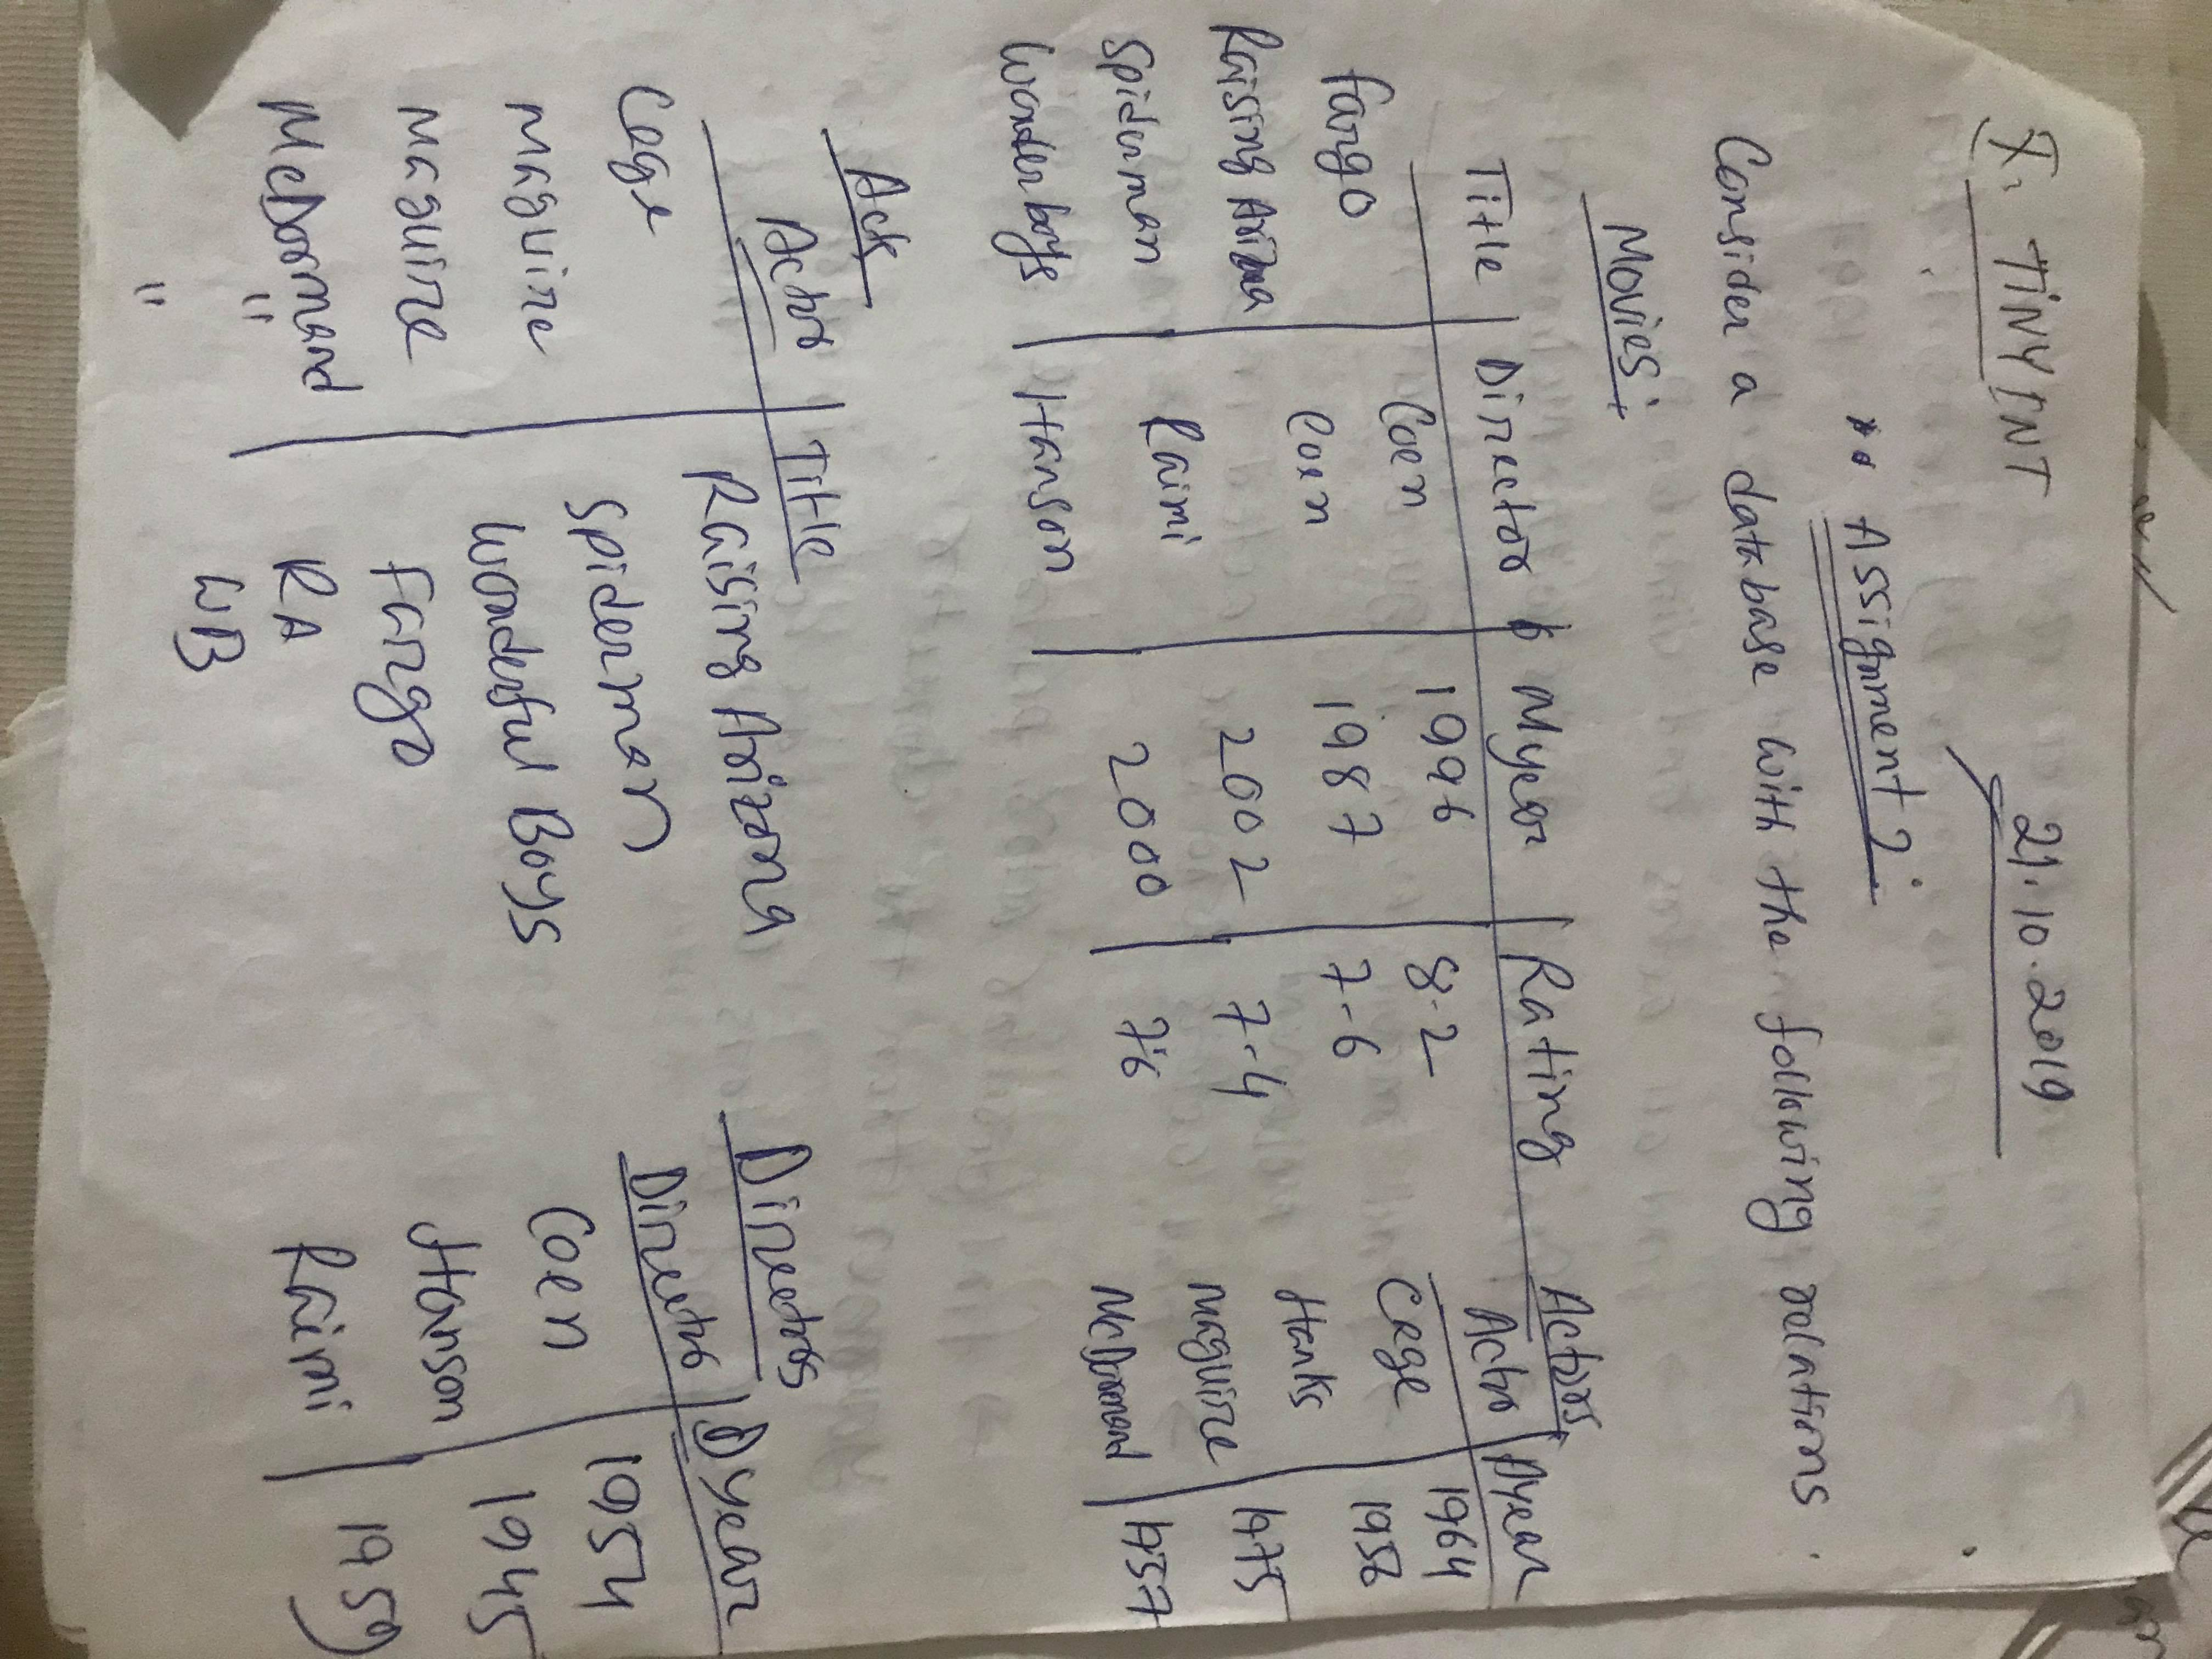
\includegraphics[scale=.3]{2.png}
\end{center}
\caption{Simulated leg \vadjust{\vskip 10mm \vskip 0pt}}
\label{fig:fig2}
\end{figure}
\end{center}
\hfill \break




\begin{center}
Graphical user interface to control a leg
\vadjust{\vskip 10mm \vskip 0pt}
\begin{figure}[h]
\begin{center}
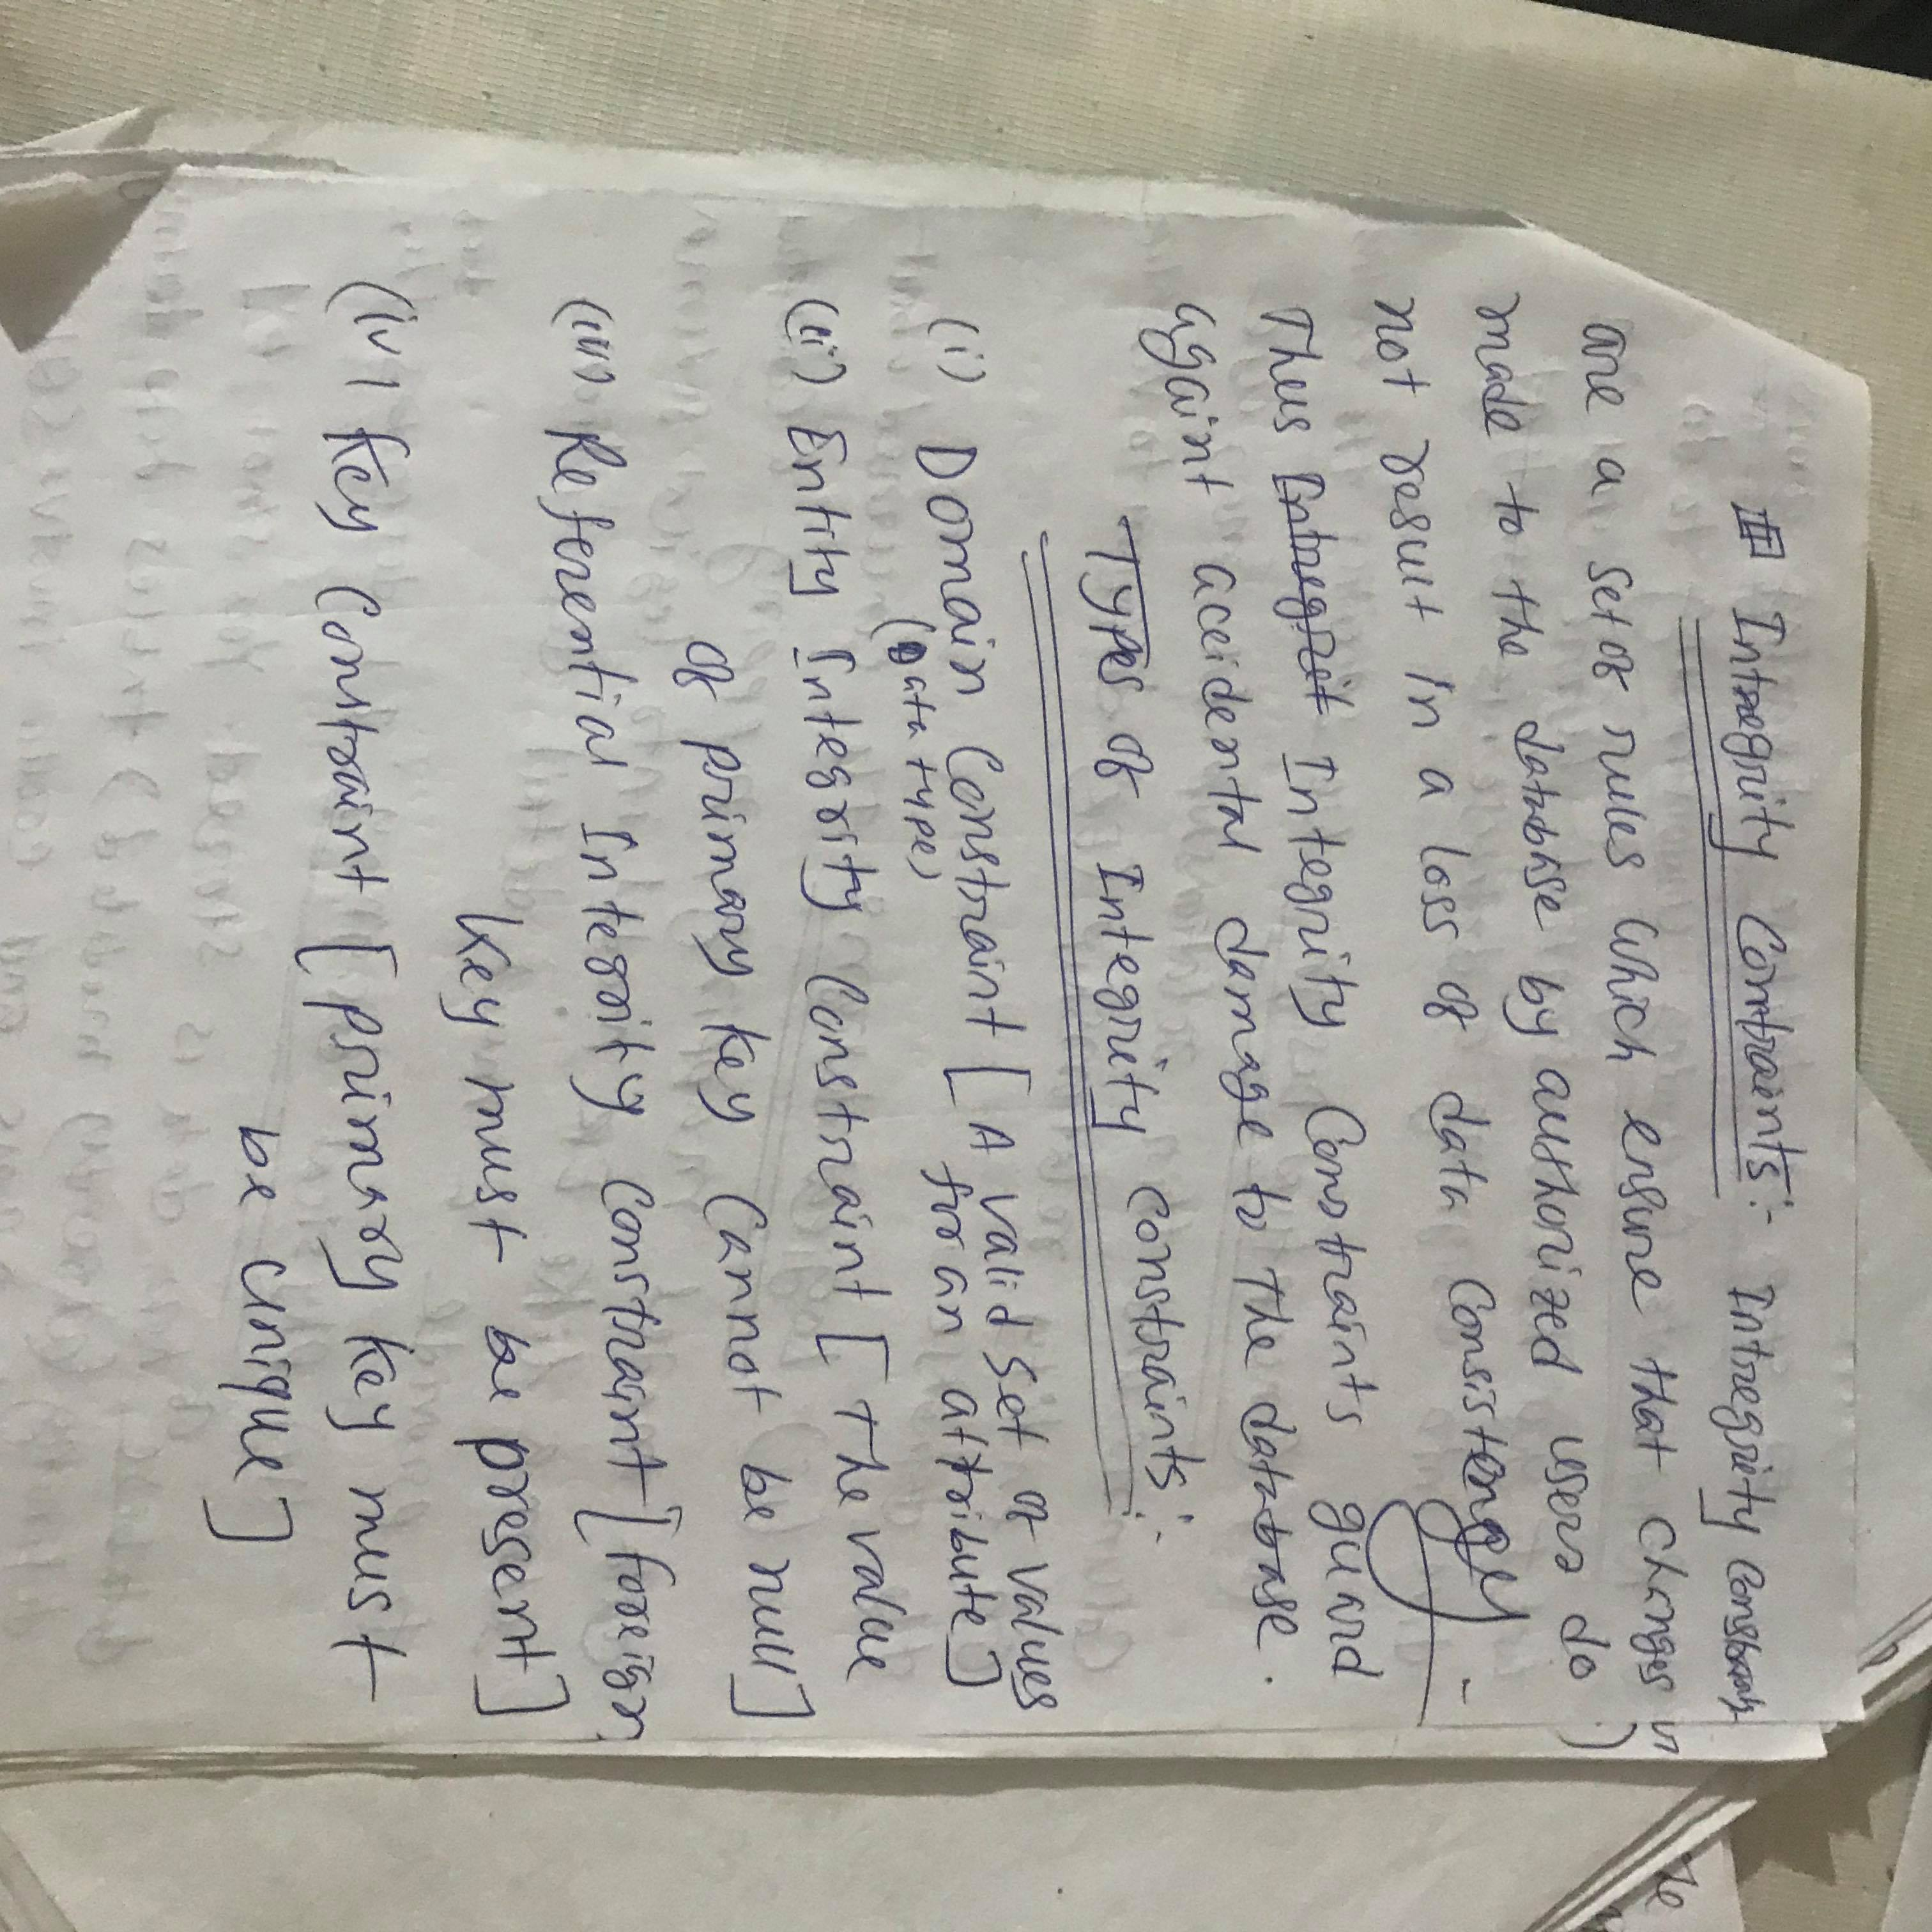
\includegraphics[scale=.3]{3.png}
\end{center}
\caption{GUI to control one leg\vadjust{\vskip 10mm \vskip 0pt}}
\label{fig:fig2}
\end{figure}
\end{center}
\hfill \break


\newpage

\subsection{Use of Inverse kinematics on my project}
After completing the implementation of forward kinematics on the simulated leg then I have write a java code to implement the inverse kinematics on this leg. 

\begin{center}
Implement Inverse Kinematics on the leg\vadjust{\vskip 10mm \vskip 0pt}
\begin{figure}[h]
\begin{center}
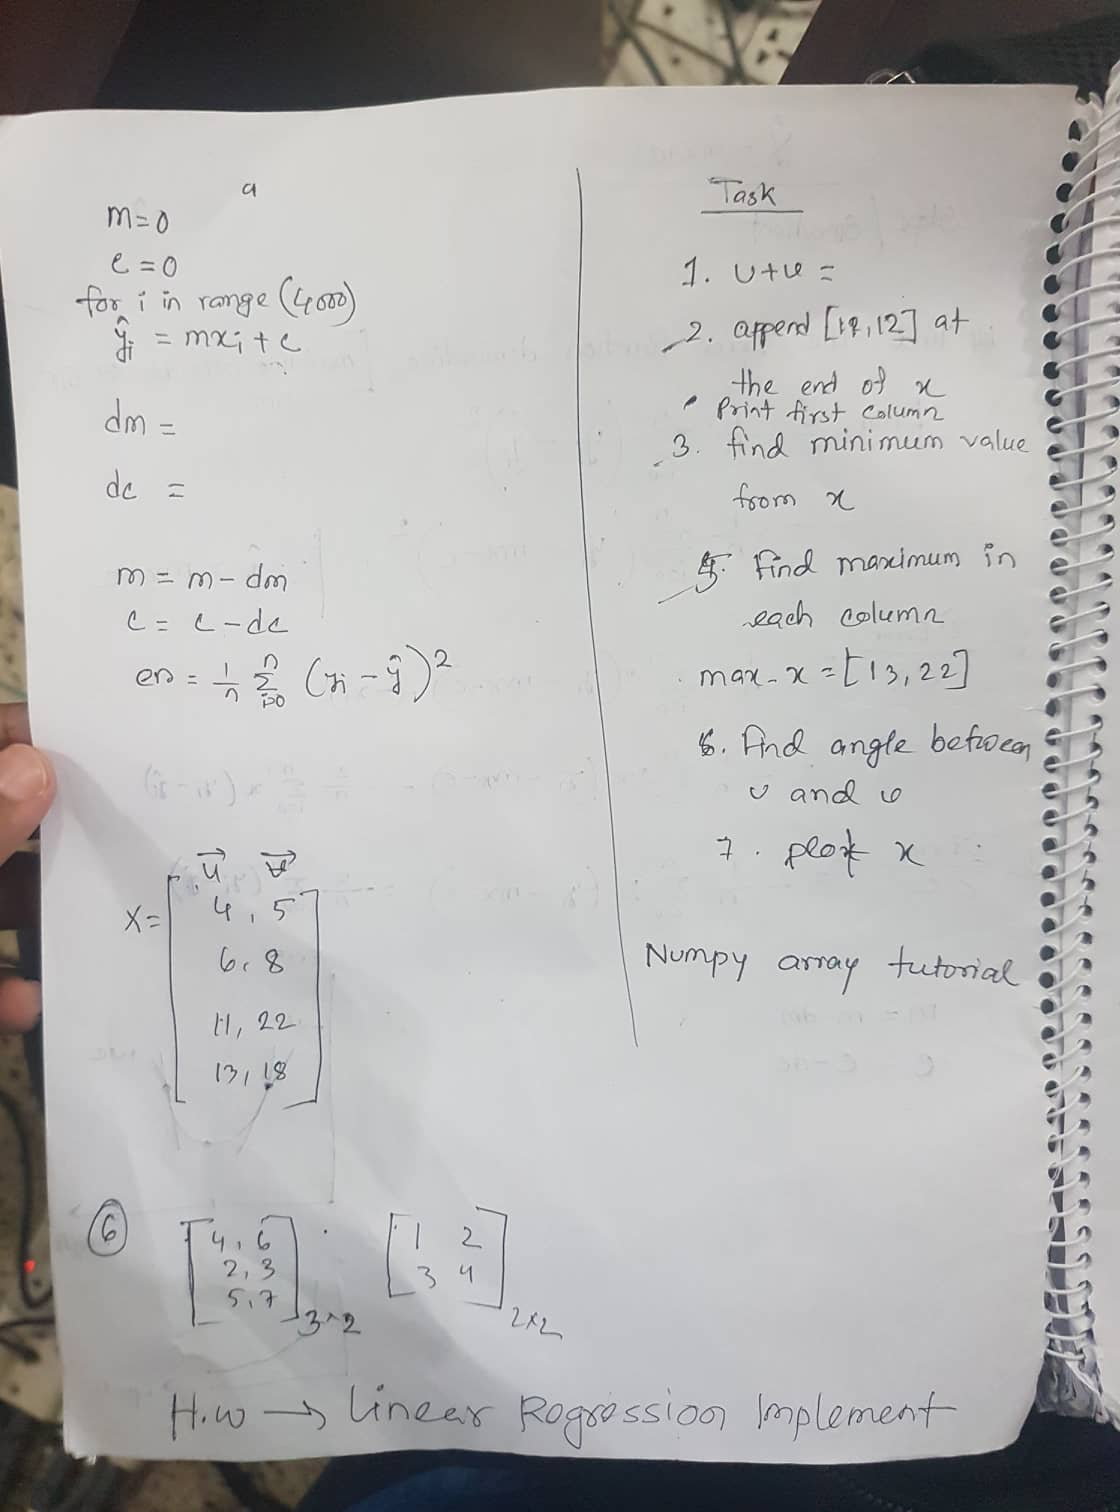
\includegraphics[scale=.3]{4.png}
\end{center}
  \caption{Inverse Kinematics implementation \vadjust{\vskip 10mm \vskip 0pt}}
\label{fig:fig2}
\end{figure}
\end{center}
\hfill \break

\newpage

\section{Software and Hardware components of this project}

\subsection{Software Part}

\begin{itemize}
\item netbeans
\item V-rep simulator
\end{itemize}
These are the software i have used in my project, for the java code implementation i have used netbeans. And for  the structural design of this robot I have used v-rep simulator.

\subsection{Hardware part}

\begin{itemize}
\item Arduino 
\item lipo battery
\item Servo motor
\item Jumper wire
\item wire 
\item pvc board
\item And other accessories
\end{itemize}
I haven't start work on hardware part yet.These are the components that I'm going to use in hardware part. 

\newpage

\section{Project Details}
After completed the implementation of forward and inverse kinematics on one leg then i have started to design the full body of the robot on v-rep. 

\subsection{Robot Design  First Part}

This is the main part of  simulation.
fist design was for one leg then i have design the full body of this robot. 


\begin{center}

this is the first design of the robot with full body
\vadjust{\vskip 10mm \vskip 0pt}
\begin{figure}[h]
\begin{center}
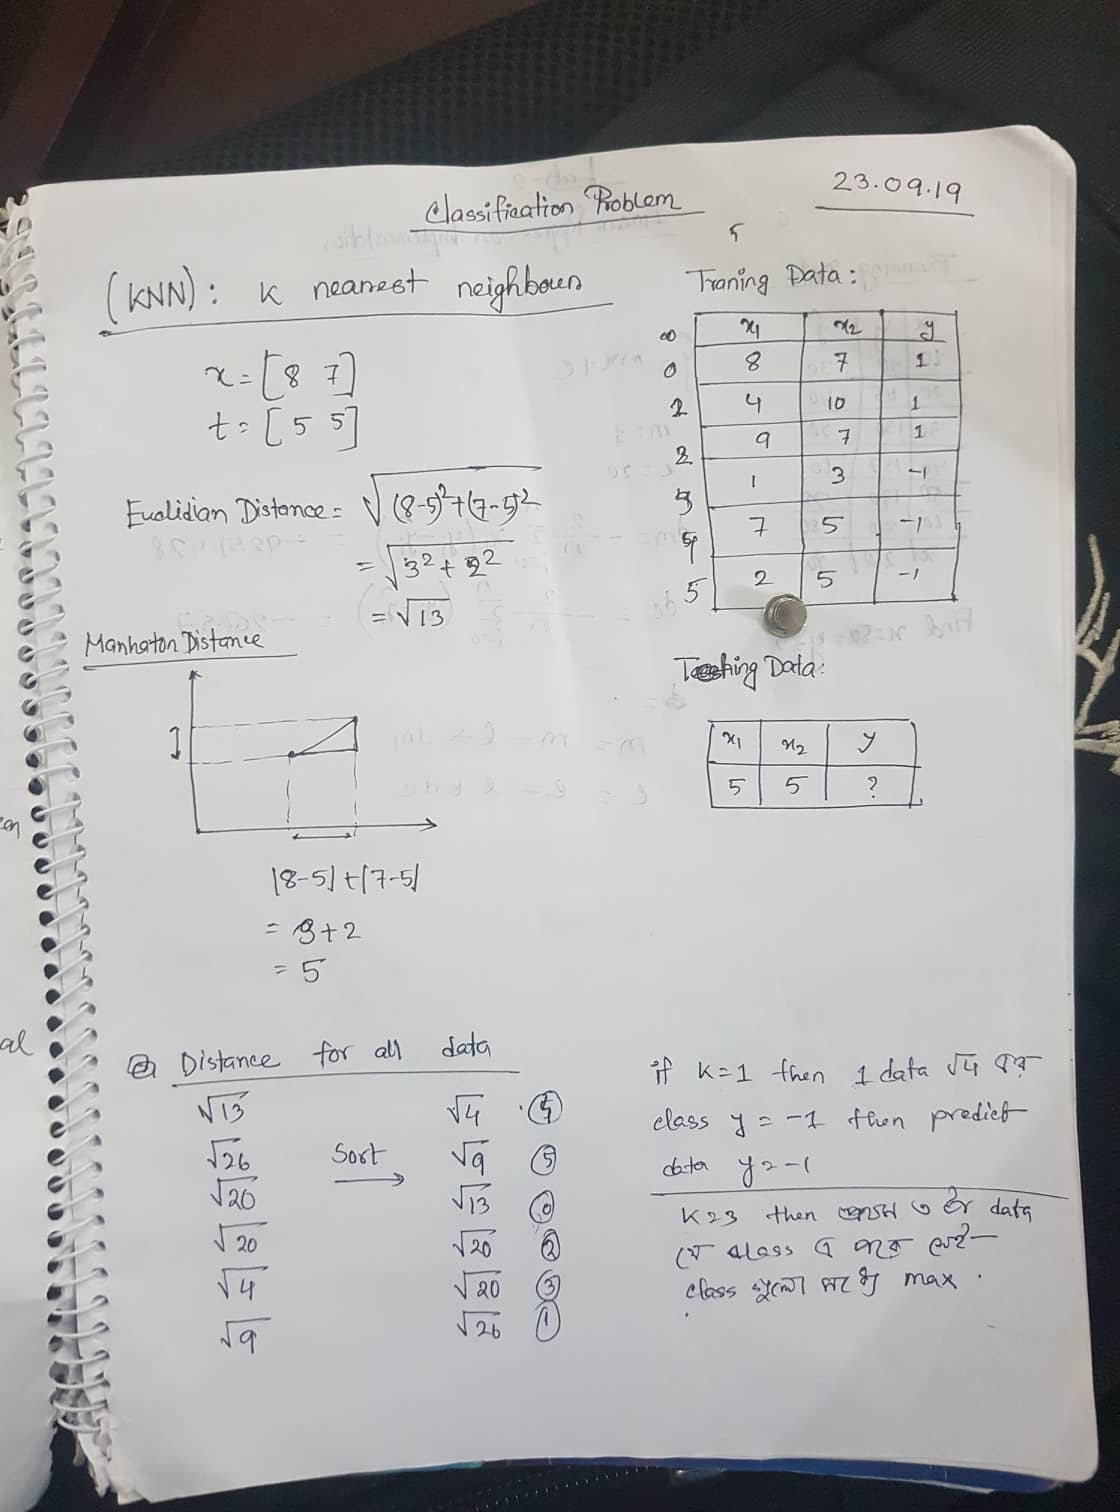
\includegraphics[scale=.3]{5.png}
\end{center}
  \caption{Full body of the robot \vadjust{\vskip 10mm \vskip 0pt}}
\label{fig:fig2}
\end{figure}
\end{center}
\hfill \break

\newpage

\subsection{Robot Design Second Part  }
There was some problem in first design.So that i have created another design to avoid those problem which i have faced on first design.This design is more efficient than the previous design. 


\begin{center}

this is the second design of the robot
\vadjust{\vskip 10mm \vskip 0pt}
\begin{figure}[h]
\begin{center}
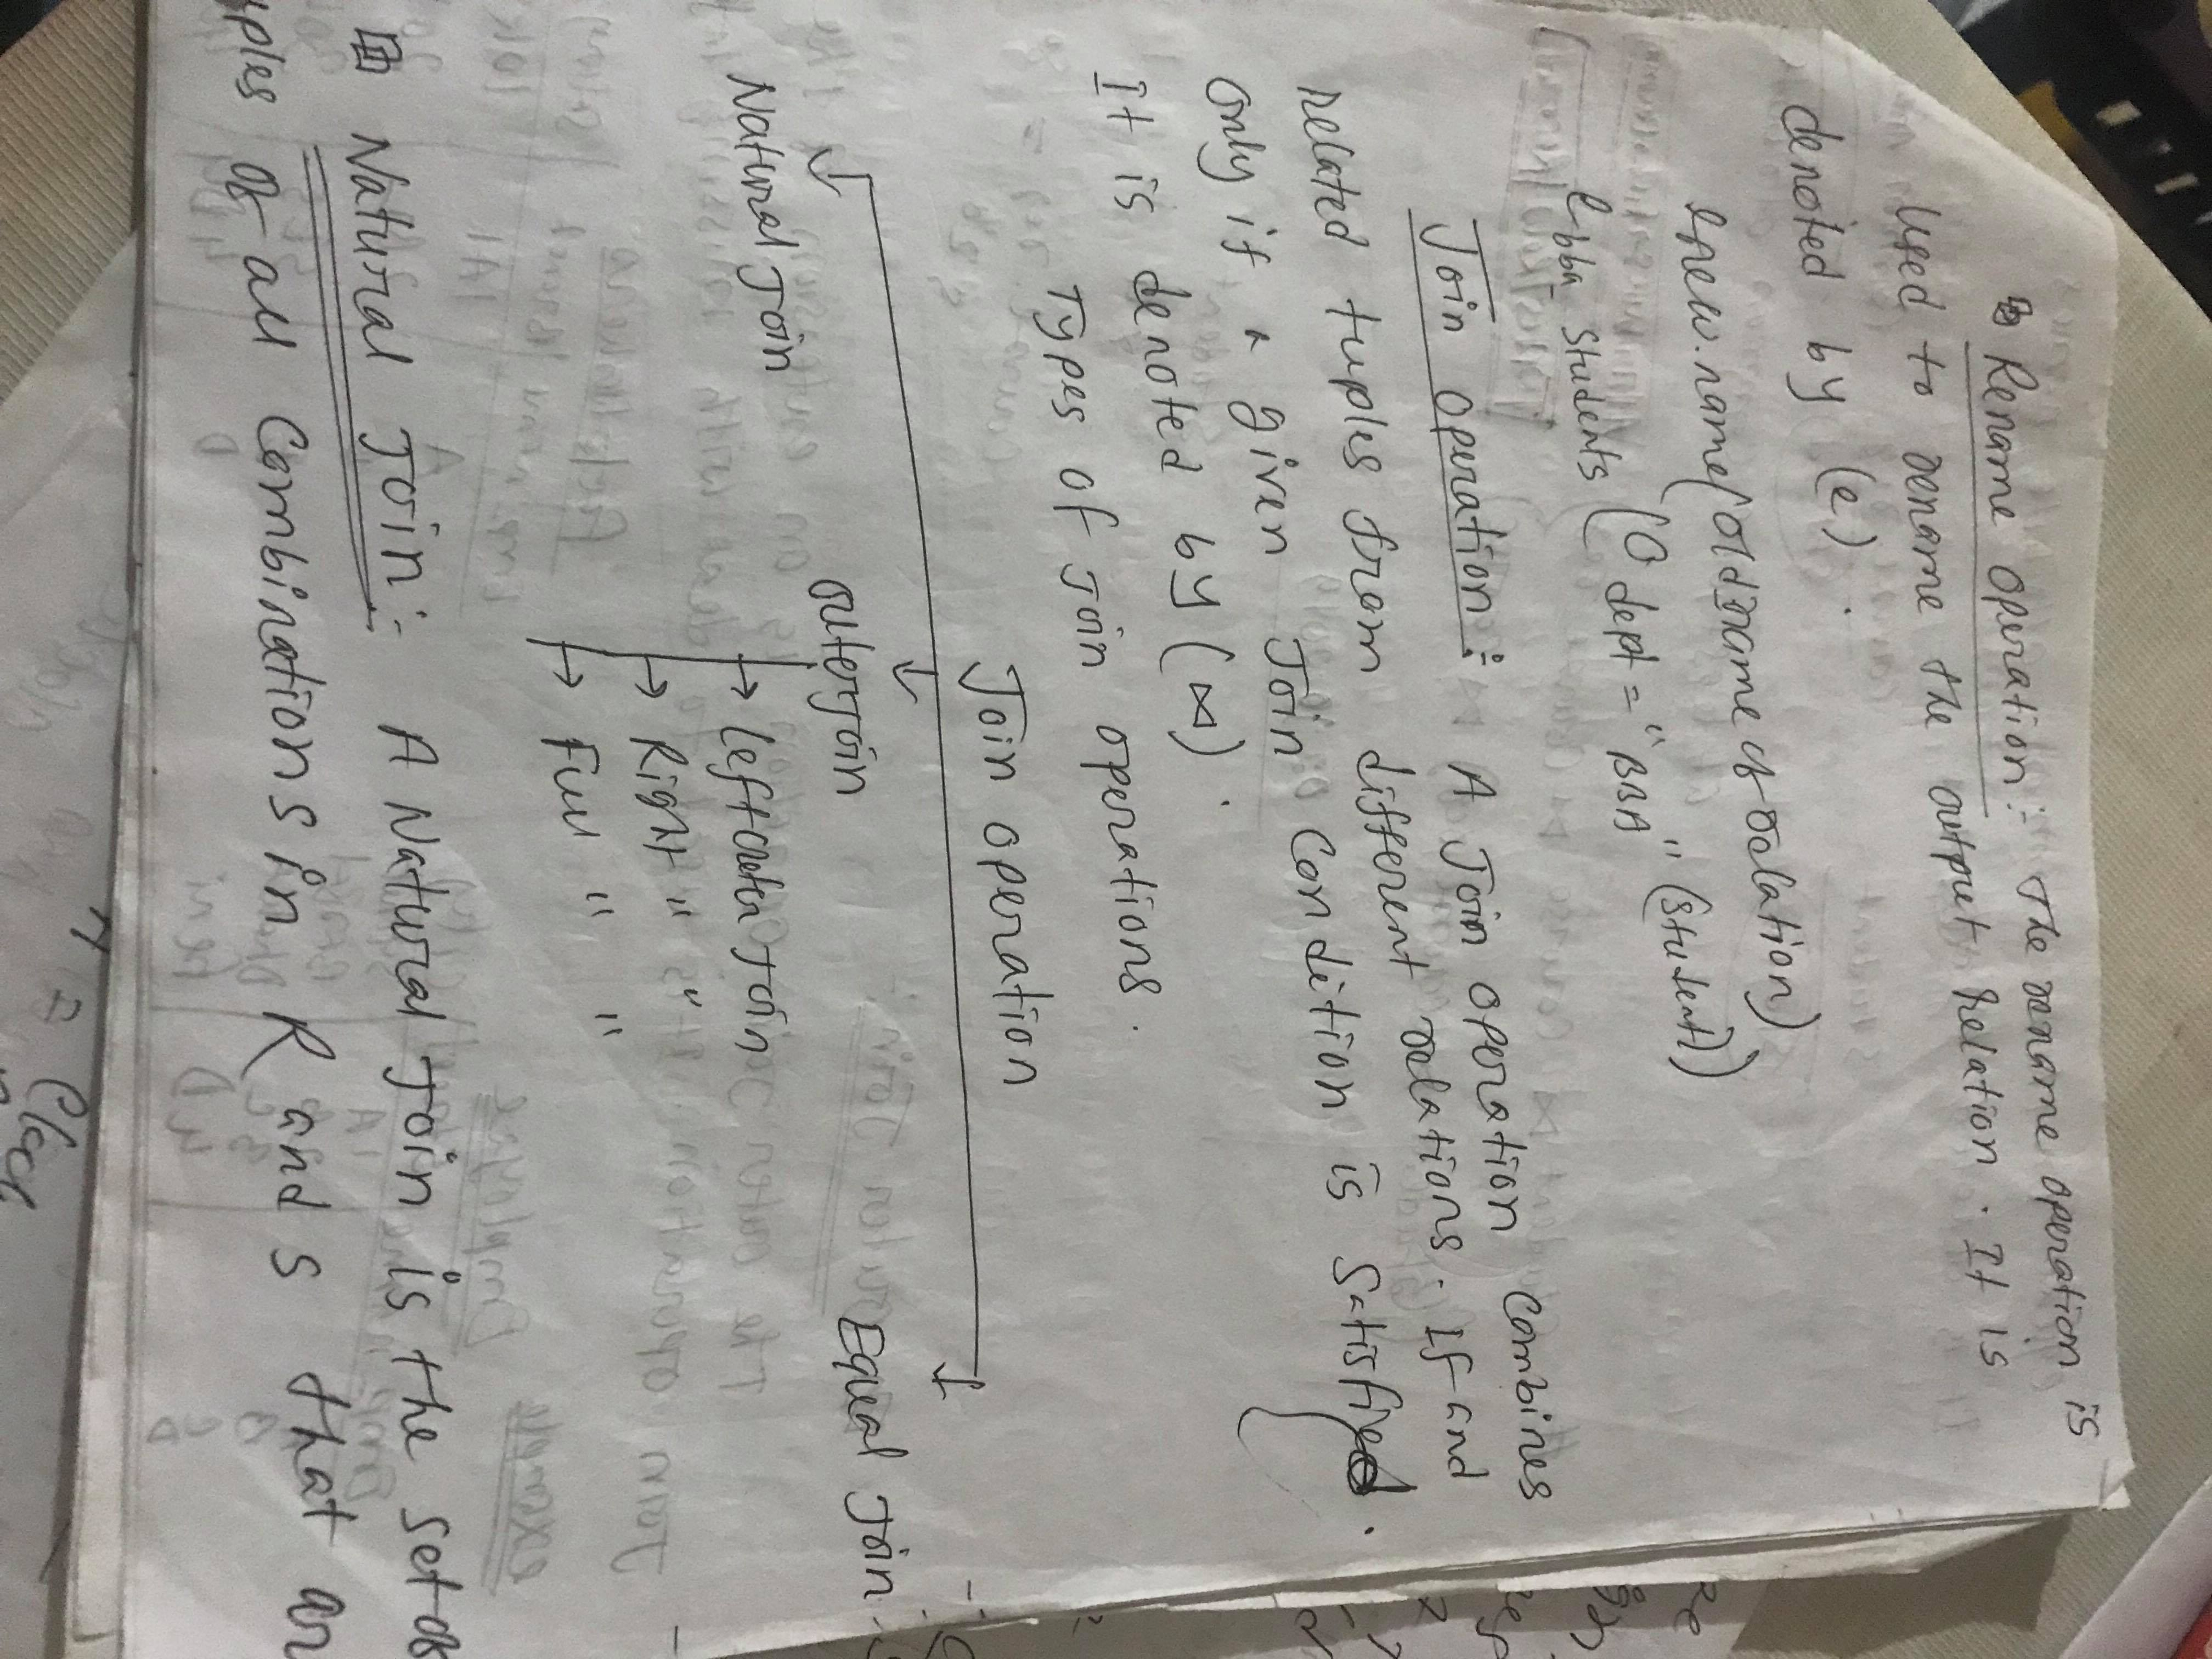
\includegraphics[scale=.3]{6.png}
\end{center}
  \caption{Second design \vadjust{\vskip 10mm \vskip 0pt}}
\label{fig:fig2}
\end{figure}
\end{center}
\hfill \break
\newpage



\subsection{Leg movements control}
After complete the design of the robot I have start to implement forward and inverse kinematics on every legs.

\begin{center}

This figure is showing the movement of right side's legs 
\vadjust{\vskip 10mm \vskip 0pt}
\begin{figure}[h]
\begin{center}
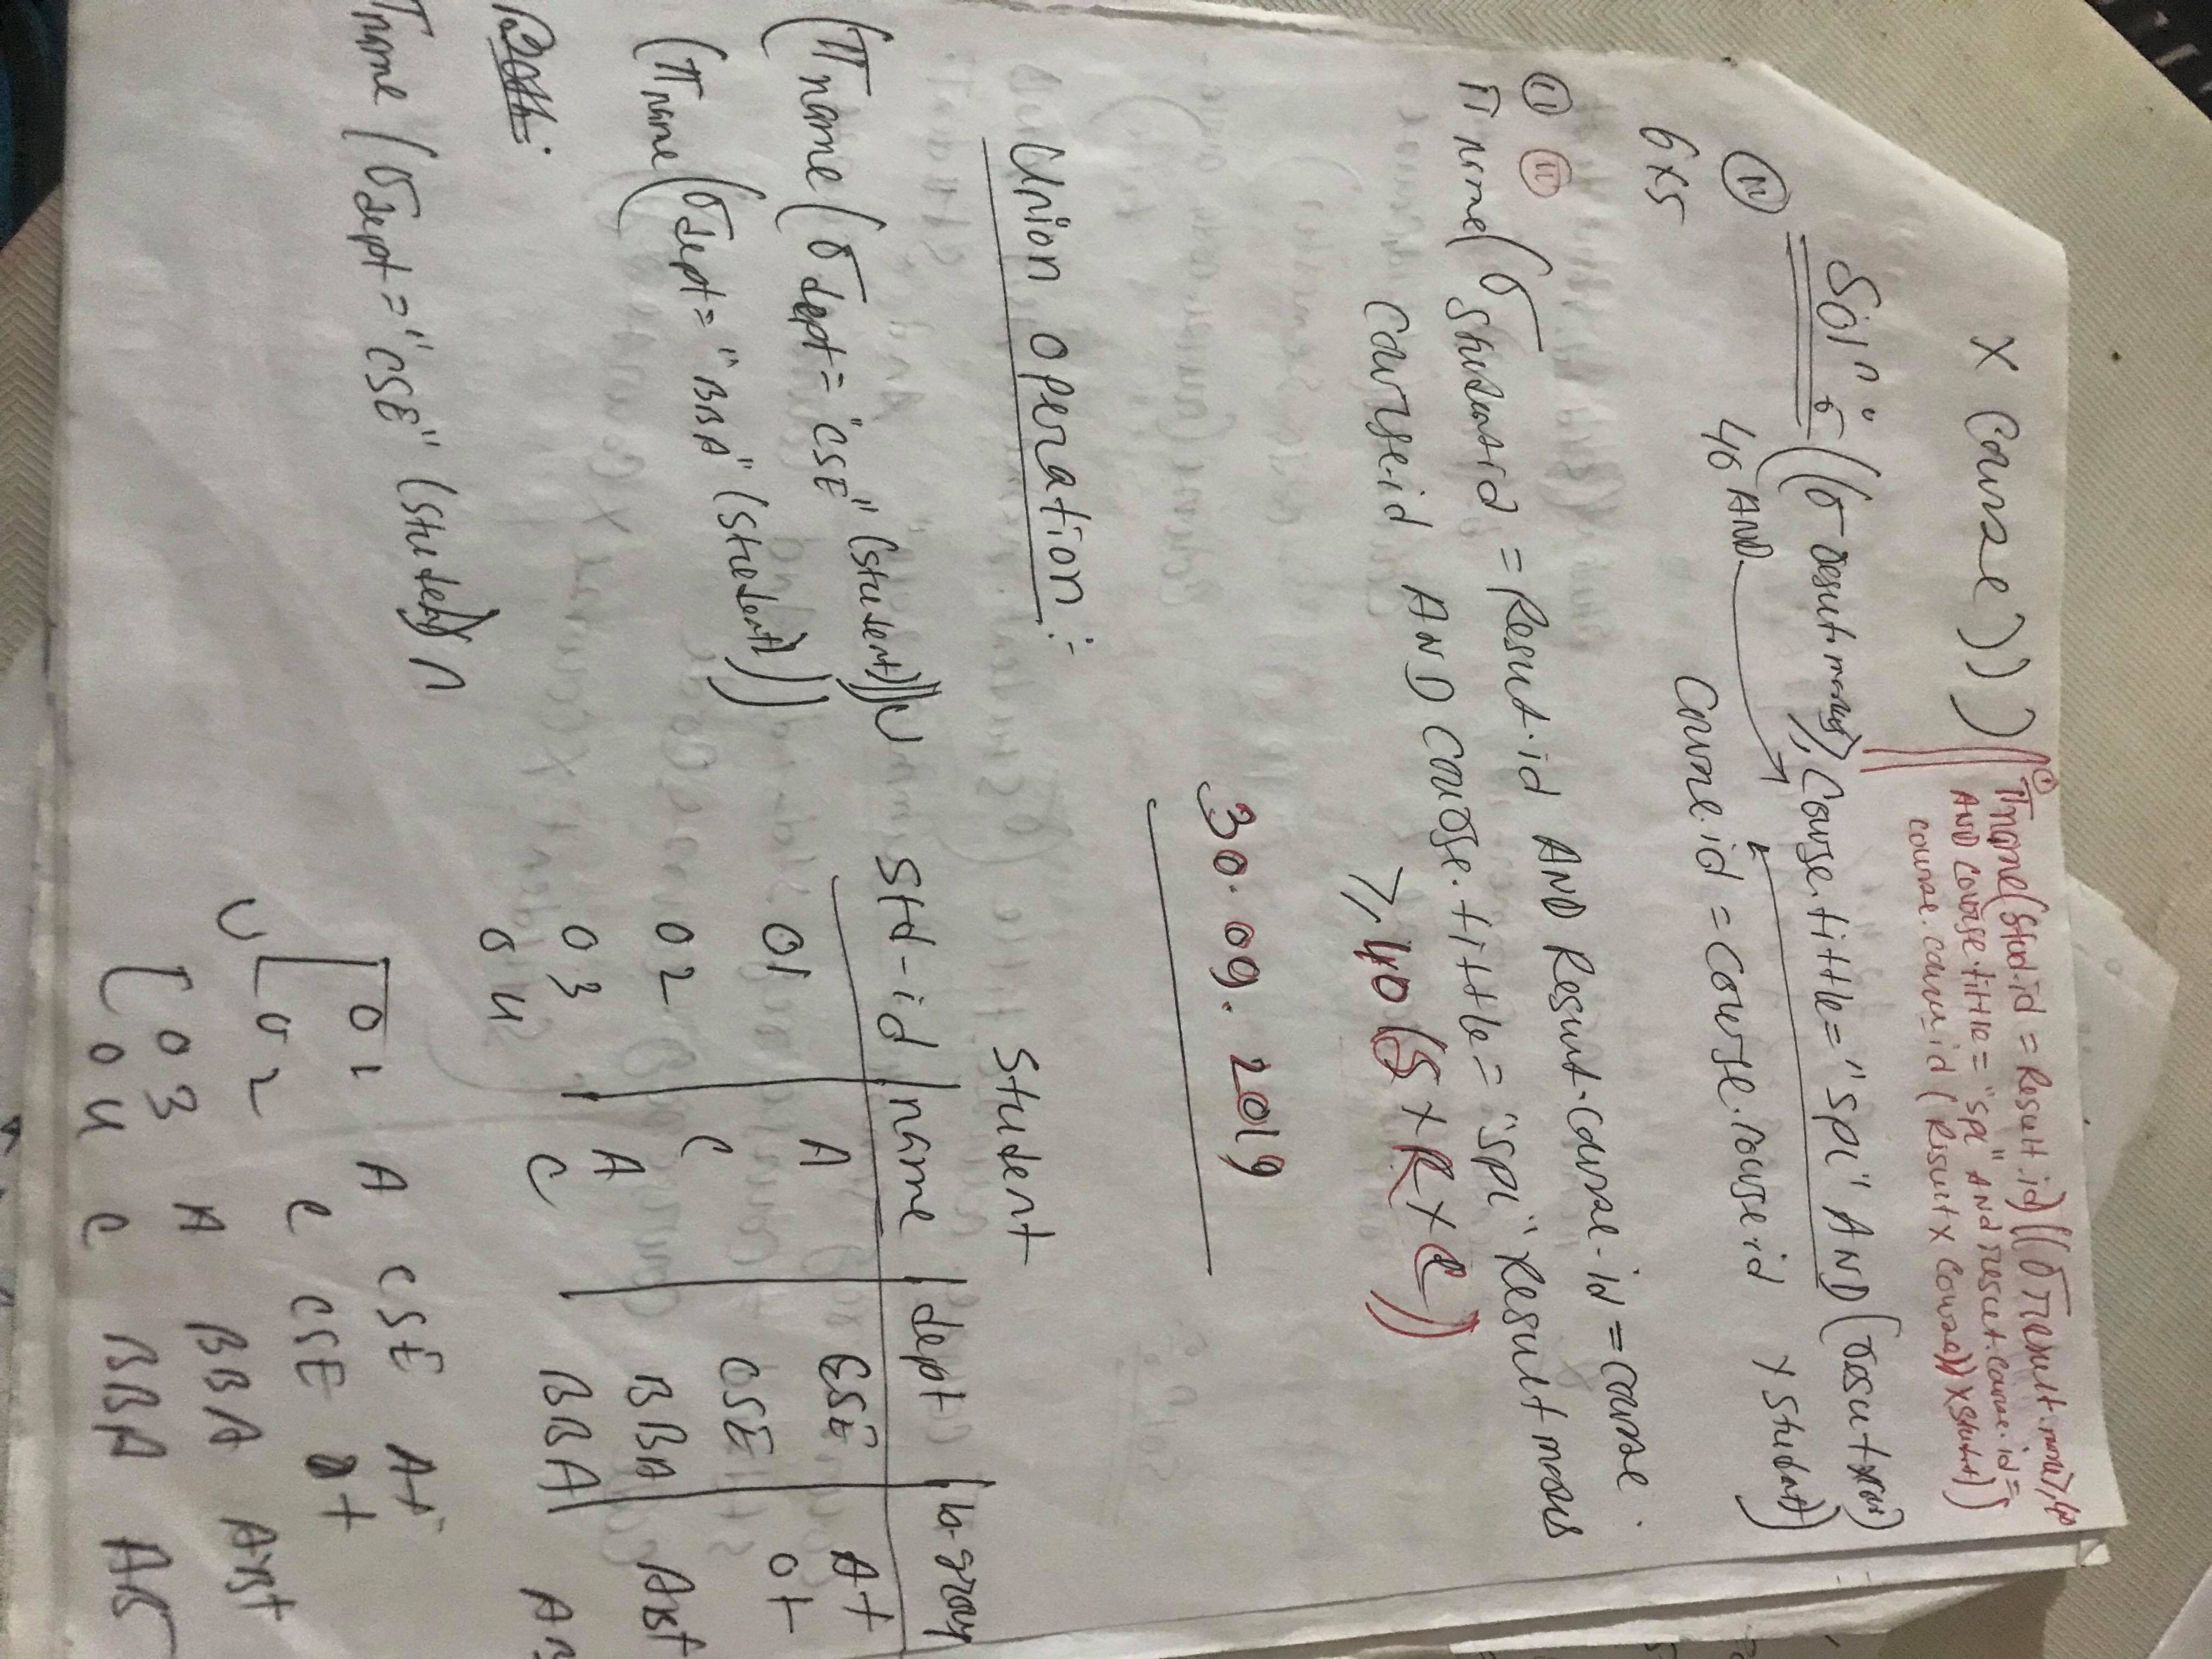
\includegraphics[scale=.3]{7.png}
\end{center}
  \caption{Right sides legs movement \vadjust{\vskip 10mm \vskip 0pt}}
\label{fig:fig2}
\end{figure}
\end{center}
\hfill \break

\newpage

Figure 8 is showing the movements of all legs of the robot.Every leg can be control individually. 

\begin{center}



This figure is showing the movement of both side's legs 
\vadjust{\vskip 10mm \vskip 0pt}
\begin{figure}[h]
\begin{center}
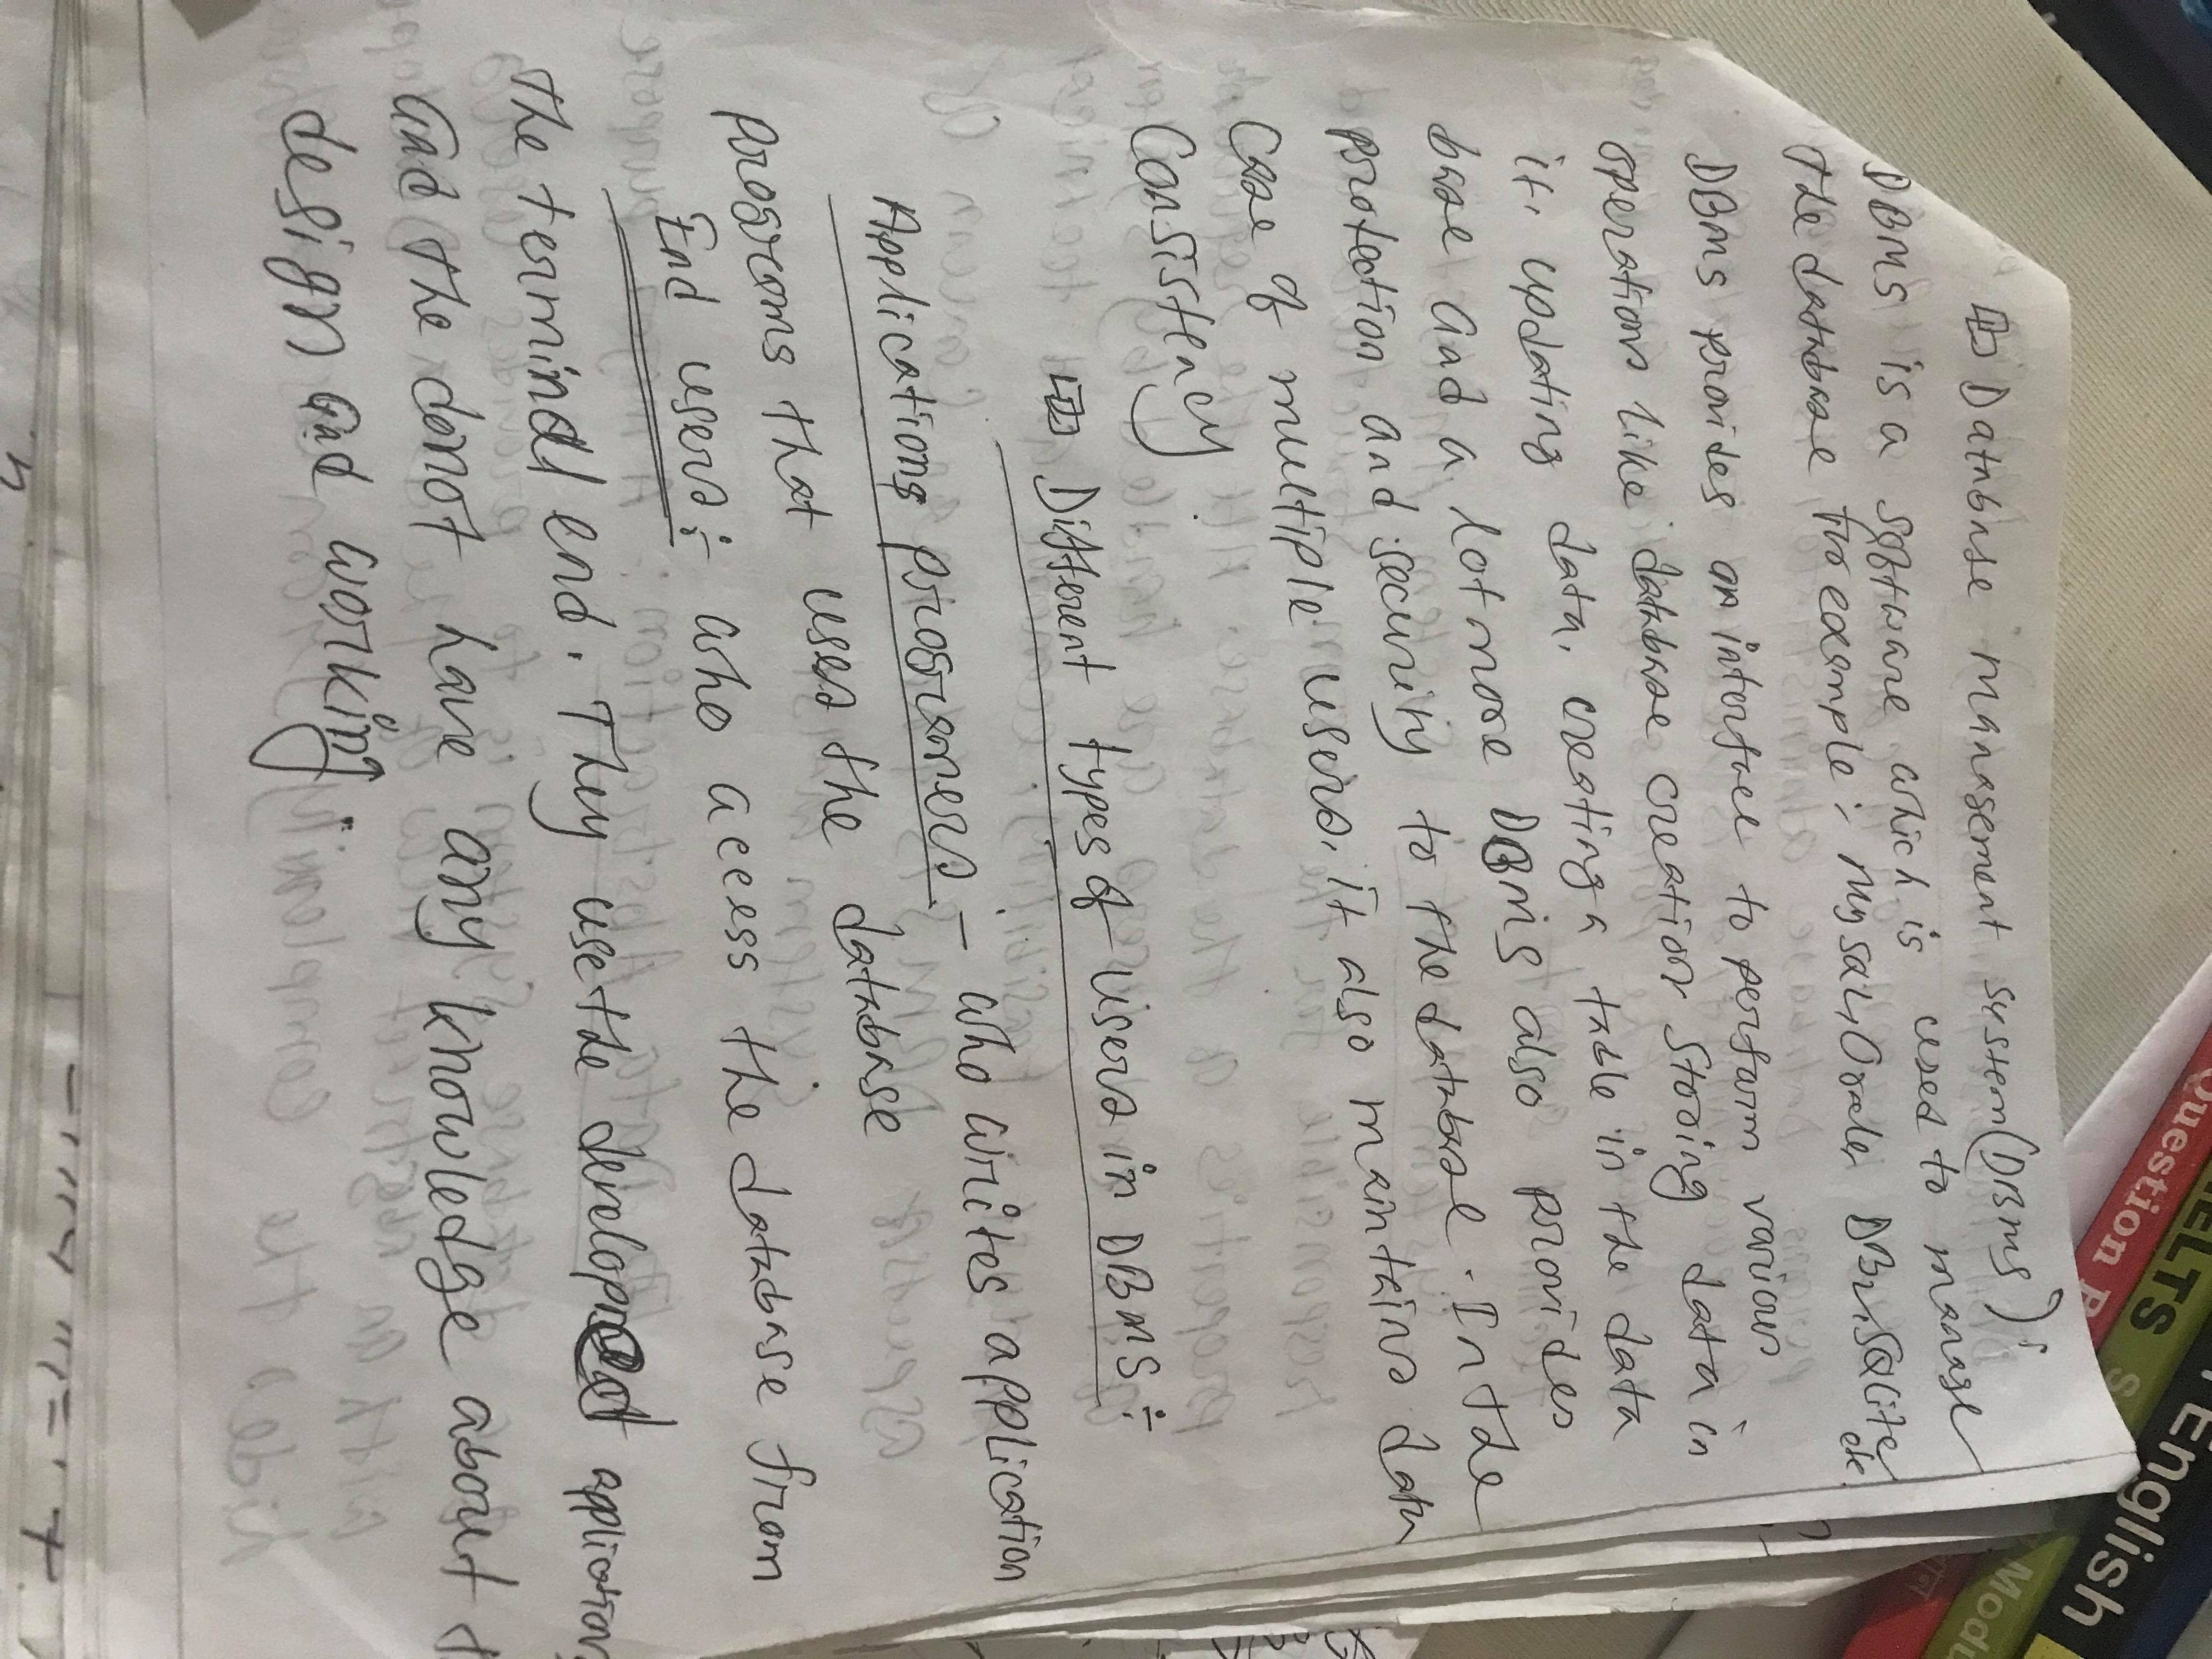
\includegraphics[scale=.3]{8.png}
\end{center}
  \caption{both sides legs movements \vadjust{\vskip 10mm \vskip 0pt}}
\label{fig:fig2}
\end{figure}
\end{center}
\hfill \break

\newpage


\section{Challenges}
That was not so easy to do design a robot on v-rep simulator cause it was new to me and I have never worked on legged robot.This is the first time that I'm working on legged robot.
\subsection{Connecting v-rep  with java netbeans}

I have face a lot of problem in this part. It took 10-15 days to connect v-rep simulator with java program.Actually I implemented all the code in wrong way.And did not add package of coppelia in java.When i implement the first program on v-rep that was so exiting, And then i realized that it's not that hard actually. 
\subsection{Design the robot}
This part was interesting I have randomly create many structure before build the actual design of the robot.But I have faced a lot of problem when I  start the build process of the robot.Because the measurement of the robot has to be perfect unless it won't work.
\subsection{Balance problem of the robot}
One of the major problem was to make this robot stable and make it perfectly balanced.And the image of that robot is given bellow

\begin{center}



This figure is showing that the robot was not stable on the ground
\vadjust{\vskip 10mm \vskip 0pt}
\begin{figure}[h]
\begin{center}
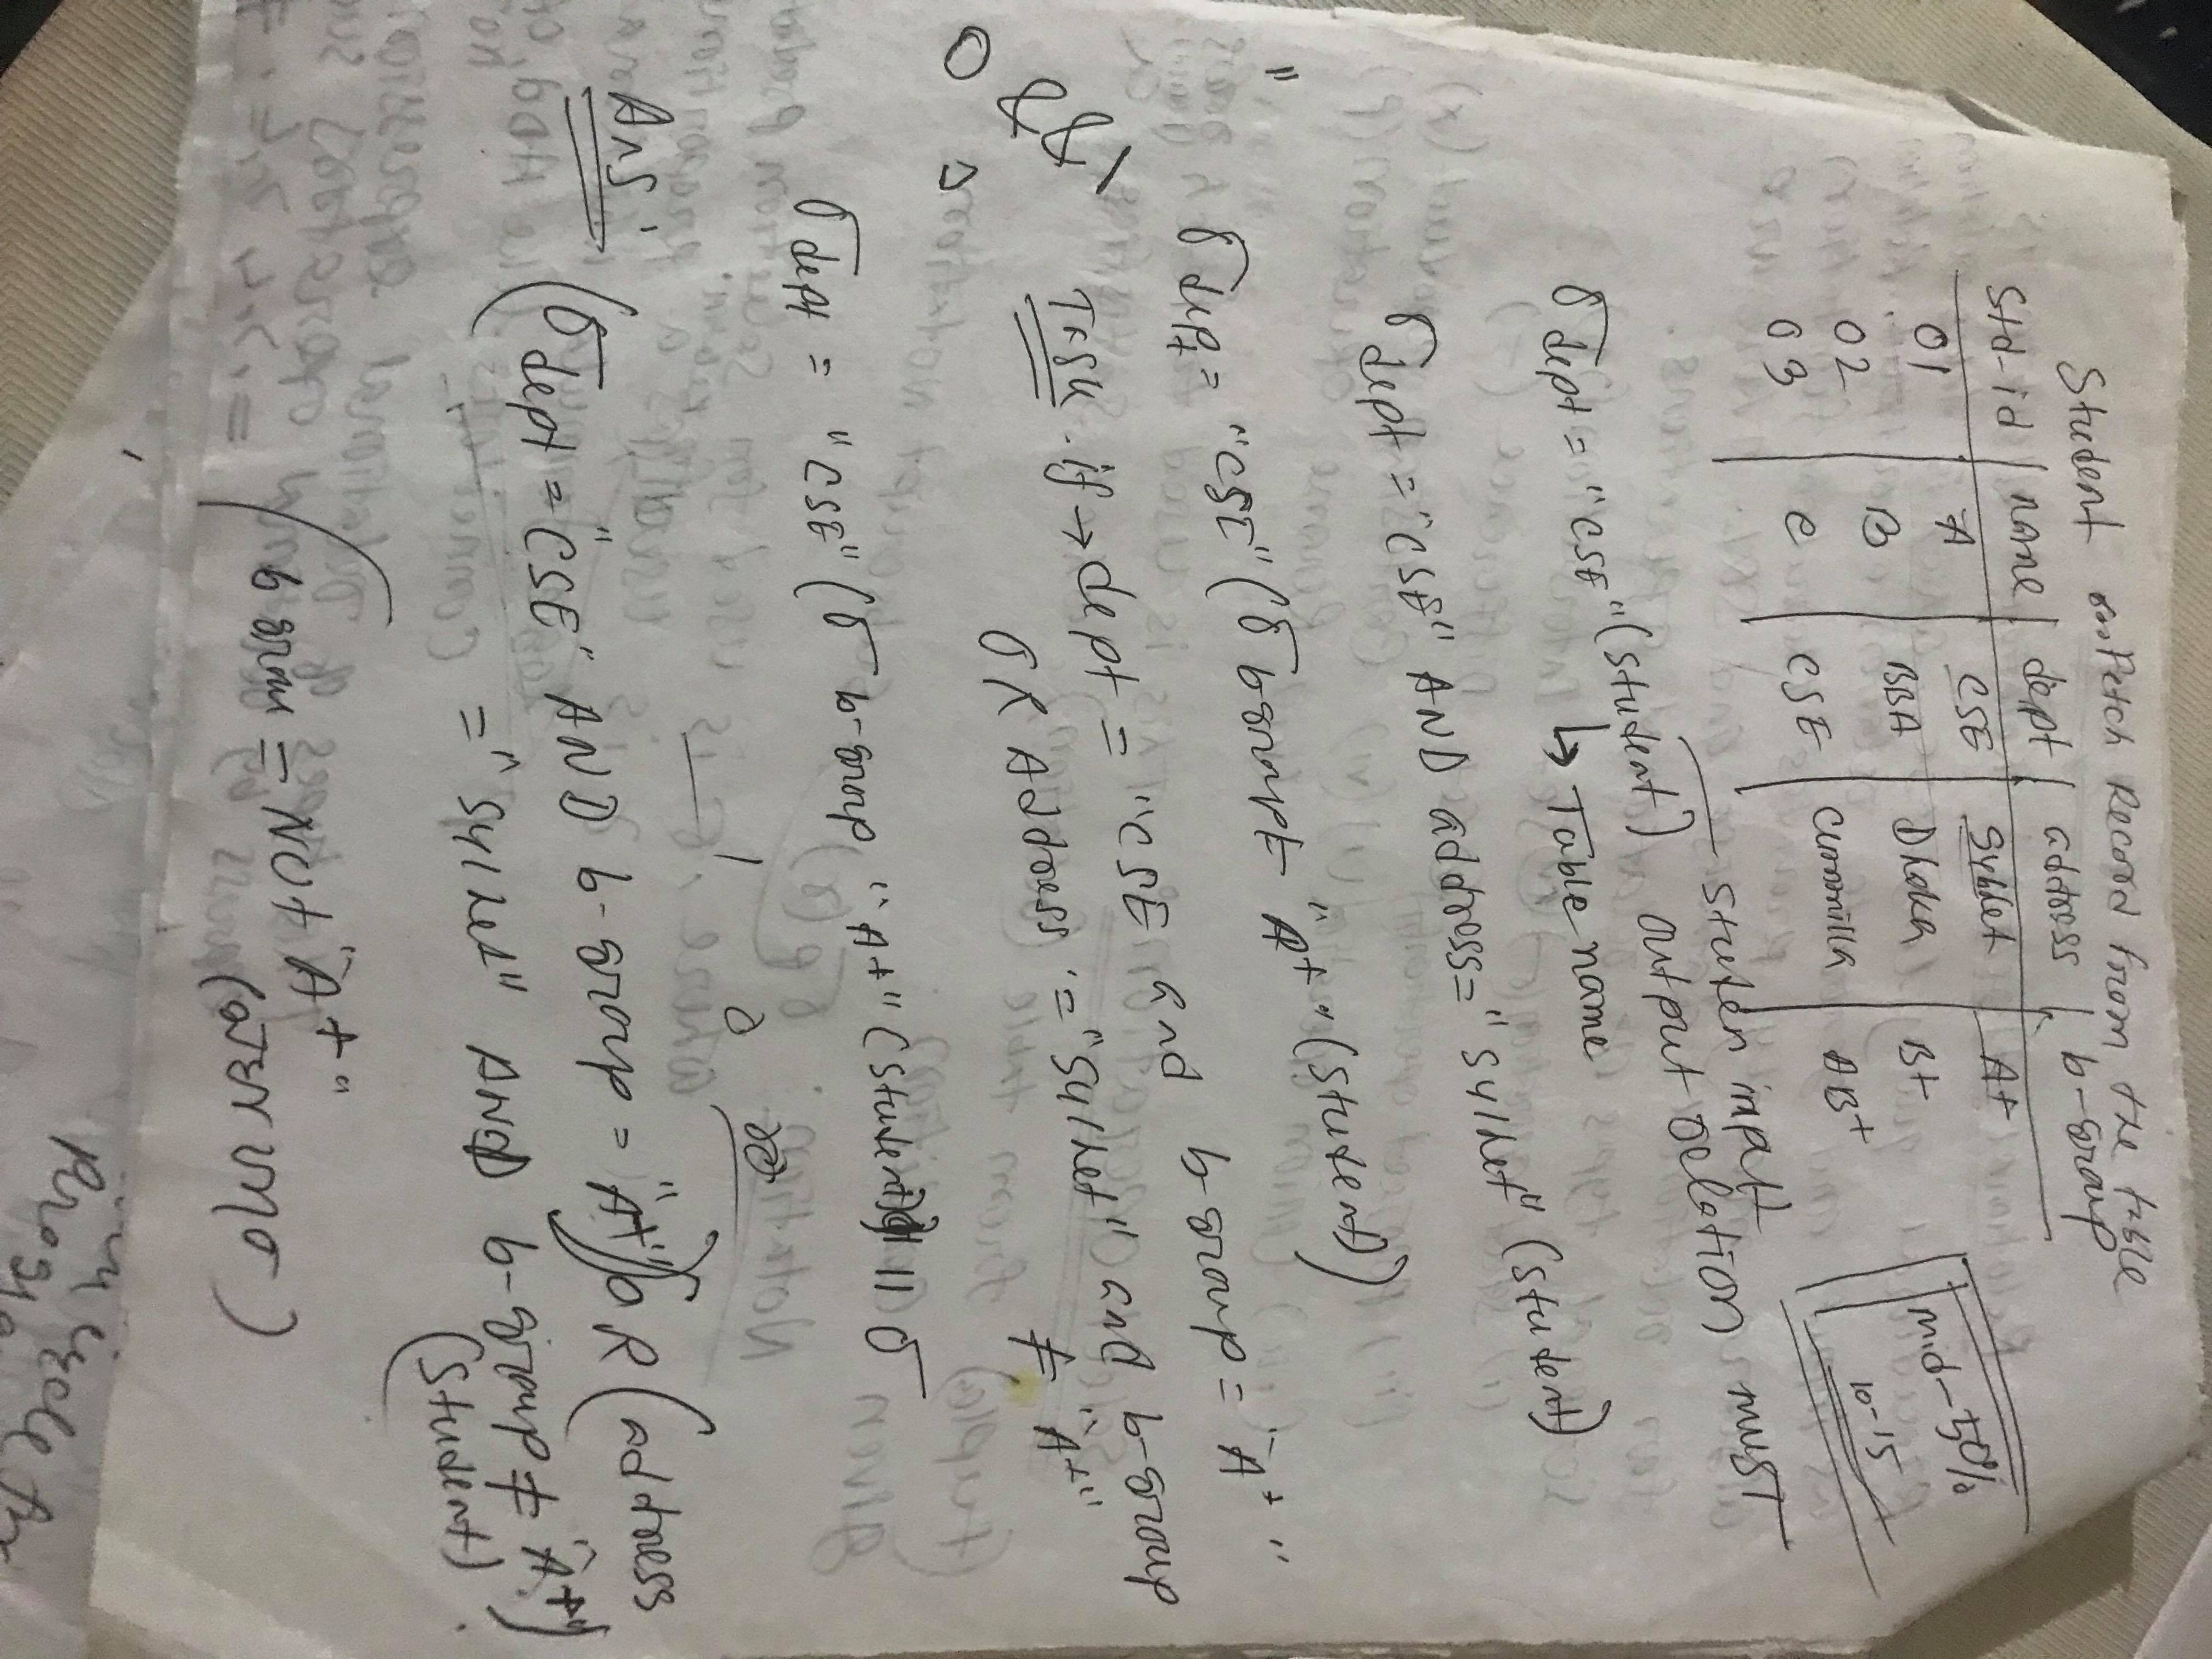
\includegraphics[scale=.3]{9.png}
\end{center}
  \caption{balance problem of the robot \vadjust{\vskip 10mm \vskip 0pt}}
\label{fig:fig2}
\end{figure}
\end{center}
\hfill \break
 
\newpage




\section{References}


\begin{itemize}
\item https://www.rosroboticslearning.com/inverse-kinematics
\item https://oscarliang.com/inverse-kinematics-and-trigonometry-basics/
\item http://www.cs.cmu.edu/~15464-s13/lectures/lecture6/IK.pdf
\item https://www.rosroboticslearning.com/forward-kinematics

\item https://en.wikipedia.org/wiki/Kinematics
\item https://www.bostondynamics.com/spot
\item http://news.mit.edu/2019/mit-mini-cheetah-first-four-legged-robot-to-backflip-0304

\item https://www.quanser.com/products/2-dof-robot/

\item https://www.hindawi.com/journals/sv/2017/2762169/


\item https://ieeexplore.ieee.org/document/8588551/

\item https://www.intorobotics.com/robotic-arm-kits-for-your-next-project/






\end{itemize}


\end{document}






